\documentclass[UKenglish]{uiomasterthesis} %% ... or norsk or nynorsk or USenglish
\usepackage[utf8]{inputenc} %% ... or latin1
\usepackage[T1]{url}\urlstyle{sf}
\usepackage{babel, csquotes, graphicx, textcomp, uiomasterfp, varioref}
\usepackage{amsthm}
\usepackage{amsmath, amssymb, amsfonts, bm}
\usepackage[backend=biber,style=numeric-comp, sorting=none]{biblatex}
\usepackage[hidelinks, hypertexnames=false]{hyperref}

\title{Explainable Artificial Intelligence for Out-of-Distribution detection}
\subtitle{Using irregularities in machine learning explanations to detect when a model is faced with unusual data}
\author{Jonatan Hoffmann Hanssen}

\addbibresource{bibliography.bib}

\theoremstyle{definition}
\newtheorem*{definition}{Definition}

\begin{document}
\uiomasterfp[dept={Department of Informatics},
program={Robotics and Intelligent Systems},
supervisors={Hugo Lewi Hammer \and Kyrre Harald Glette},
long]

\frontmatter{}
\begin{abstract}
Here come 3--6 sentences describing your thesis.
\end{abstract}

\begin{xabstract}[Sammendrag]
Here comes the abstract in a different language.
\end{xabstract}

\tableofcontents{}
\listoffigures{}
\listoftables{}

\begin{preface}
I would like to thank my dog.
\end{preface}

\mainmatter{}
\chapter{Introduction}

\section{Motivation}

Machine Learning generally, and Deep Learning specifically, have seen a tremendous increase in performance in recent years, performing comparable to humans in tasks such as image classification, speech recognition and many others \cite{performance}. Consequently, DL methods have been deployed in a multitude of fields and have become a part of our daily lives through their role in web search, text translation, computer vision and in many other technologies which are taken for granted. In medicine, deep learning has the potential to provide faster and more accurate detection of diseases by being trained on cases from thousands of previous patients \cite{xaisurvey}. Despite this, "surprisingly little in health care is driven by machine learning" \cite{dlmed}.

% TODO: make these citations more specific

To explain this discrepancy, we should consider that despite their impressive performance, deep learning methods are not without their flaws. Firstly, deep neural networks are inherently unexplainable due to the large number of parameters that any non-trivial network has. State of the art models will perform millions of operations to evaluate a single data point, and it is therefore impossible for humans to comprehend and explain the entire process which lead the model to make a particular decision. In medicine, this is a major limitation of deep learning methods, as both doctors and patients expect to be able to understand why a decision was made \cite{tingsim}.

Secondly, although neural networks may attain high accuracy on test data and appear to have learned great insights about the tasks they are employed in, they often lack robustness and can suffer large drops in performance on data points which are slightly different from the training data. As \cite{intriguing} has shown, it is possible to create data points which are imperceptibly different from normal data points, yet still fool otherwise high performing models. More problematically, unlike humans, who recognize when they are faced with a novel situation where their expertise might be lacking, DL methods will predict equally confidently on data points which are far outside the data they have been trained on \cite{tingsim}.

These two problems lead to the fields of Explainable Artificial Intelligence (XAI), and Out-of-Distribution (OOD) detection. XAI attempts to explain the reasons why a model came to a decision, which helps to remedy the black-box nature of complicated DL models. In a healthcare setting, such explanations can be inspected by medical practitioners to confirm the diagnosis, and can be used to give patients information about why decisions regarding their health were made. OOD detection attempts to uncover when a data point is too different from the training data to be classified reliably. These methods could alert medical practitioners when such data points occur, thus avoiding potentially fatal misclassifications.

Both of these fields have seen increased interest in recent years, and are vital parts of any integration of DL in medical settings. This thesis will focus on OOD detection, but will attempt to use methods inspired by XAI to improve detection performance. The overarching intuition is that by inspecting the explanation of a model on a specific data point, we may be able to uncover flaws or irregularities in the explanation which could help us determine whether the data point is OOD.

% This thesis will attempt to combine the two fields, by using methods inspired by XAI to improve OOD detection.

\section{Problem Statement}

As explained in the previous segment, OOD detection is a developing field, which has become more important in recent years as machine learning is being used for higher impact tasks, such as disease detection. Finding novel methods which improve a model's ability to detect when input is OOD is important to increase the robustness of machine learning models as they are used in these real-world scenarios. The field of XAI is concerned with understanding the inner workings of a model, and could thus offer insights which could help us detect unusual behaviour in the model as a result of OOD data points. The problem statement is thus as follows:

\textbf{Can methods inspired by the field of Explainable Artificial Intelligence be used to improve Out-of-Distribution Detection?}
\\

To answer this question, I introduce 3 objectives:

\begin{enumerate}
  \item Give a thorough introduction to the fields of XAI and OOD detection
  \item Develop an effective and theoretically sound OOD detection method which is inspired by insights gained from the field of XAI
  \item Perform experiments to measure the performance of this new method in comparison current State-of-the-Art OOD detection methods
\end{enumerate}

\section{Scope}

Use only post-hoc methods, pretrained resnet models. Use well established OOD datasets first for comparisons. Then focus on medical datasets, hyperkvasir and maybe more. Only use open-source programs. Python and Pytorch. Mainly focus on images. Probably only CNN models, as a lot of XAI is based on that. Maybe also try methods that work on vision transformers as well, but then we are more restricted to post-hoc methods probably.

\section{Research Methods}

Use ACM


\section{Main Contributions}

Objective 1 is accomplished in chapter \ref{chapter:background}. Here, the fields of XAI and OOD detection are introduced, their respective taxonomies are explained and a selection of specific methods are explained in more detail. This chapter provides a good entry for machine learning researchers who wish a decent introduction to the two fields. Objective 2 is achieved in chapter \ref{chapter:newmethod}. Here, I introduce the groundbreaking NEW METHOD, which achieves a FPR95 of 1\%, blowing all previous methods out of the water. Objective 3 is accomplished in chapter \ref{chapter:experiments}, where we confirm that NEW METHOD is insanely good.

\section{Outline}

Chapter \ref{chapter:background} gives a short introduction to machine learning, followed by a deeper look at the fields of XAI and OOD detection. The different datasets which will be used in chapter \ref{chapter:experiments} are also introduced, among them the HyperKvasir gastrointestinal dataset \cite{hyperkvasir}. Chapter \ref{chapter:newmethod} introduces NEW METHOD. Chapter \ref{chapter:experiments} tests NEW METHOD against State-of-the-Art methods within the field of OOD detection. The tests are first conducted on well known OOD datasets, and then in a more specialized medical setting using the HyperKvasir dataset. After the experiments follow a discussion and conclusion in chapters \ref{chapter:discussion} and \ref{chapter:conclusion}.

\chapter{Background} \label{chapter:background}

This chapter gives a short introduction to important concepts in the field of machine learning generally, followed by a more in depth look at the fields of OOD detection and XAI. Finally, the datasets used in chapter \ref{chapter:experiments} are covered.

\section{Machine Learning}

Machine Learning is the field of algorithms that are able to learn from data, as opposed to being explicitly programmed. Such algorithms use statistical methods to learn relationships in data, and use these relationships to generalize to unseen data. More formally, \cite{mitchell} gives the following definition of machine learning algorithms:

\begin{definition}
A computer program is said to learn from experience $E$ with respect to some class of tasks $T$ and performance measure $P$ if its performance at tasks in $T$, as measured by $P$, improves with experience $E$.
\end{definition}

Thus, machine learning is a different paradigm from traditional problem solving, where programs are made to solve problems by following explicit rules. For example, a traditional image classification system attempting to differentiate between malignant and benign tumors might use hand-crafted rules which consider the texture, color and size of a tumor. As one might imagine, such rules will quickly become very complicated when we consider all the possible factors which might influence the appearance of a tumor. Using a machine learning approach, we would instead feed an algorithm with thousands of images of both benign and malignant tumors, and the algorithm could then be automatically updated until it predicted the correct category with a high enough accuracy.

Machine Learning is commonly divided into the three subcategories of supervised, unsupervised and reinforcement learning

% A simple comparison is between the two chess engines Stockfish and AlphaZero. Stockfish plays chess by evaluating possible moves according to metrics created by humans\footnote{This is actually no longer the case, as the classical evaluation has been replaced by a neural network (a machine learning approach), however, I will pretend that it still is for the sake of argument}, such as valuing a Queen as equivalent to nine pawns and a 

\subsection{Supervised Learning}

Supervised Learning is a subcategory of machine learning where we have a dataset containing both inputs and desired outputs. In the example above, we could use supervised learning by creating a dataset of images of tumors (the input) and corresponding labels which indicate whether each tumor is malignant or benign (the desired output). The learning goal of the algorithm is then to associate images with the correct label. Because we know the correct answer, we are able to fine-tune the algorithm automatically whenever it makes a mistake. However, supervised learning requires labeled data, which can be very costly, especially in the medical domain, where deciding whether a tumor is malignant or benign requires expert knowledge.

\subsection{Unsupervised Learning}

In unsupervised learning, we do not have any labels. In these cases, we might not know whether data points belong to different classes or not. Instead, we can use machine learning to uncover patterns in the data, for example by attempting to cluster the data into different groups and seeing if these groups are sufficiently separated. An example use case could be for fraud detection in a bank. By feeding financial transaction from many different users into an unsupervised learning model and asking it to perform clustering of the data, it might be possible to find a group of users whose transactions differ substantially from the rest, which might indicate that their transactions are fraudulent.

\subsection{Reinforcement Learning}

Reinforcement Learning deals with problems where we do not know exactly what the correct solution is, but we are able to assess whether a given solution is good or not. For example, when controlling a robot arm, it is difficult to say exactly what angles each joint should be for every millisecond when picking up an object, but if the arm does not pick up the object, we know the algorithm has failed. In these problems, the algorithm is trained through reinforcement, where good attempts are rewarded and bad attempts punished.

\section{Neural Networks}

Neural Networks are a class of machine learning algorithms, which have become the clear state of the art in almost all fields where machine learning is applied. Notable examples are computer vision, image classification, speech recognition, text and image generation and machine translation. Neural networks are loosely inspired by our own brains, where neurons are connected together and send information between each other. By connecting thousands of neurons together, neural networks are able to learn complicated relationships between the input and output.

\subsection{Feed Forward Neural Networks}

A Feed Forward Neural Network (FFNN), also known as a Multilayer Perceptron, traces its roots to the very beginning of machine learning through the work of Frank Rosenblatt \cite{rosenblatt}. It forms the basic structure for neural networks which has been adapted and modified over the years to form more complex architectures such as convolutional, recurrent or residual neural networks. The basic structure of an FFNN is that the input values are passed through an affine transformation (a matrix multiplication followed by the addition of a bias), and then passed through an activation function, which produces outputs. These outputs can then go through the same process again, which constitutes a single "layer". By stacking several of these layers, with non-linear activation functions, an FFNN is able to learn arbitrarily complex mappings between inputs and outputs\footnote{In fact, by the Universal Approximation Theorem, only a single hidden layer between the input and output is necessary, although this theorem does not give a way to construct such a network for any given function}. Mathematically, a single layer can then be described as follows:

\begin{equation}
\bm{x_{i+1}} = \sigma_i (A_i \bm{x_i} + \bm{b_i})
\label{ffnn}
\end{equation}

Here, the input $\bm{x_i}$ is linearly transformed by the weights of the matrix $A_i$ from the input space to the output space, then each value of the new vector in the output space is adjusted by an addition of a bias term, and finally an activation function ($\sigma_i$) is applied to each value. 


\subsection{Convolutional Neural Networks}

FFNNs have some problems which make them unsuitable for working with high dimensional, spatially connected data such as the pixels which make up an image. Firstly, each input of a FFNN is connected to every output of the following layer. If we want an image.

\section{Explainable AI} \label{xai_intro}

Below follows a thourough introduction to XAI, as well as detailed look at some important methods for explainability for neural networks applied to images.

\subsection{The motivation for XAI}

Given the impressive performance of DL methods, one might be convinced that these models do not need to be explainable or interpretable, and that we instead should just place our faith in the model without knowing exactly how it came to a decision. However, as \cite{doshivelez} points out, "a single metric, such as classification accuracy, is an incomplete description of most real-world tasks". Small differences between the data distribution when the test data was collected and when the model is deployed may have a large impact on the model's performance, or the model may have learned artifacts or specificities in the training dataset which were also present in the test dataset, leading to a false belief that the model has gained generalizable knowledge when it has not. By using explainable methods, we may reveal these shortcomings.

XAI is also especially important whenever the model is used in settings where its decisions have a high impact. If a model is used by a hospital for disease detection, both the patient and doctor will probably want to be able to understand why the model has found that a disease is present. For them, high performance on a test set of different cases may not be enough. As \cite{xaisurvey} states, "for the regulated healthcare domain, it is utmost important to comprehend, justify, and explain the AI model predictions for a wider adoption of automated diagnosis". In other high impact areas, such as autonomous driving, the impact of wrong decisions by the network can have fatal consequences, and customers and regulators will want to be absolutely sure that the models used are robust and base their decisions on relevant factors as opposed to quirks in the training data. Furthermore, the right to an explanation of an automated decision affecting a person is included in the EU's General Data Protection Regulation, which states that "In any case, such processing should be subject to suitable safeguards, which should include specific information to the data subject and the right [...] to obtain an explanation of the decision reached after such assessment and to challenge the decision." \cite{gdpr}.

\subsection{Taxonomy of XAI}

This sections goes through three axes which define an XAI method:

\begin{itemize}
  \item Intrinsically explainable models versus post hoc methods
  \item Model dependent versus model agnostic methods
  \item Global versus local explanations
\end{itemize}


\subsubsection{Intrinsically explainable models versus post hoc methods}

Intrinsically explainable models are models which have sufficiently low complexity, such that it is feasible for a human to understand them without further modifications. Examples of such methods are linear regression, logistic regression and decision trees \cite{molnar}. 

Post hoc methods are methods which are applied to the model after training. These methods do not aim to constrain the model to be interpretable, but inspect the model after training. For example, after using a convolutional neural network to classify a CT-scan of a tumour (which gave a prediction of malignant), we could run post hoc algorithms on the network which are able to extract which part of the image contributed the most to the prediction. Thus, post hoc methods remove the need for the model to be simple enough for a human to understand by extracting the relevant information for us.

\subsubsection{Model dependent versus model agnostic methods}

Model dependence/agnosticity denotes whether an XAI method uses specifics of a particular type of model to generate the explanation, or whether the method can generate an explanation without using specifics of the model at all. Explanations based intrinsically explainable models are clearly model dependent, while methods that only use the input and output of the model instead of looking at the internal operations are model agnostic. An example of a model dependent method (which is not simply an intrinsically explainable model) is Class Activation Mapping, which requires a CNN with a specific architecture to function, while an example of a model agnostic method are Shapley values, which use the inputs and outputs to calculate the marginal effect of a single feature on the output value.

\subsubsection{Global versus local explanations}

Global explanations provide general relationships between the input features and outputs learned by the model over the entire dataset \cite{xaioverview}. In this way, they can show how a specific feature affects the output in general, instead of just how it affects the output of a single point. These methods are ideal for finding trends in the data, but may not be suitable for a patient wanting an explanation for their specific case.

Local explanations do not describe general trends, but focus only on a single data point. These methods give insight into how the features influenced the prediction of a single data point, but these relationships may not hold for other data points, and as such these methods do not give the same insight into the general behaviour of the model.

\subsection{Specific methods}

The following section goes through several specific XAI methods, specifically ones related to images.
\\


\subsubsection{Class Activation Mapping (CAM)}

CAM \cite{cam} is a model dependent, post hoc XAI method, which is used on Convolutional Neural Nets (CNNs). For a specific output node of a model (for example, the one denoting the presence of a specific class, such as "cat"), CAM outputs a heat map showing which areas of the input image contributed to this node. In this way, CAM gives a visual explanation to which parts of an image the model focused on when making a decision to classify an image to a specific class. This method is model dependent, because it requires a specific architecture in the final layers of the network to work.

CAM is a relatively simple method to understand. It exploits the fact that various convolutional layers of CNNs actually behave as object detectors, even when the training objective is classification \cite{cam}. As \cite{lenet5} explains, the earlier layers "extract elementary visual features such as oriented edges, end-points [or] corners", which can be used by subsequent layers to detect higher-order features. In this manner, the final convolutional layer will detect very high level visual features, combining the extracted information from all the previous layers. This layer is composed of several feature maps, where each map can be thought of as denoting the presence of some specific feature across the original image. The authors perform global average pooling (GAP) on these feature maps, giving a single value for each map, which is followed by a single dense layer and the Softmax activation function. In this way, each output node in the final layer is a weighted sum of all the global average pooled feature maps from the final convolutional layer. This means that we can represent the areas of the image which were used to perform the classification by performing the same weighted sum on the actual feature maps instead, which gives us a heat map which we can overlay on the original image (after upsampling the feature maps).

Figure \ref{camimg} shows the process visually. From this we can see that the resulting Class Activation Map (bottom right) gives an intuitive explanation for why the image in the top left gives a high score for the presence of the class "Australian Terrier".

\begin{figure}[h]
\centerline{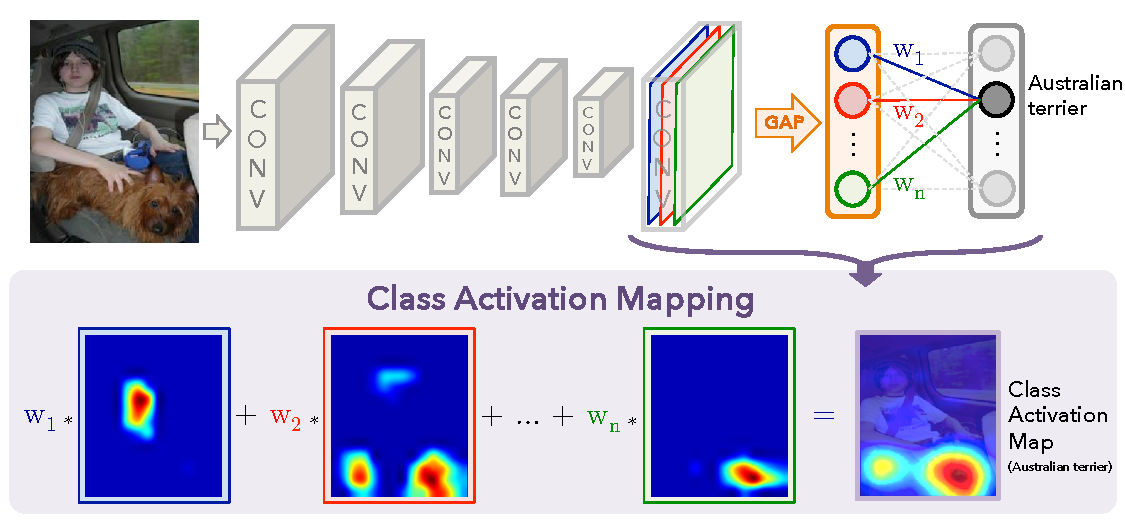
\includegraphics[width=3.25in]{figure/cam.pdf}}
\caption{Figure taken from \cite{cam}, showing the steps required to create a Class Activation Map}
\label{camimg}
\end{figure}

Although CAM is an intuitive and effective method of visualizing the inner workings of a CNN, it has some downsides. Firstly, it is highly model dependent, requiring that the model only have a single dense layer after the convolutions. Although there are some state of the art models which only use a single dense layer, this still places a limit on what models can be used, or requires the simplification of models that use more than a single dense layer. \cite[4]{cam} notes a 1-2\% drop in classification performance when performing this simplification. Secondly, the output of CAM is simply a weighted sum of all the feature maps after the final convolutional layer. As we move deeper in a CNN, we reduce the spatial resolution by downsampling, while increasing the number of channels (increasing the depth of the output while reducing the height and width). Because of this, the CAM will have a drastically lower resolution than the original image, often less than $10 \, x \, 10$, while the input image may be hundreds of pixels in both dimensions. Because of this, CAM can only show general areas, as opposed to pixel wise explanations.
\\

\subsubsection{Gradient Class Activation Mapping (Grad-CAM)}

Grad-CAM \cite{gradcam} is an improvement on CAM, which generalizes the method to function with any CNN architecture, thus making the method much less model dependent and avoiding the performance drop incurred when simplifying the model with CAM. Instead of using the weights of a final layer to calculate a weighted sum of feature maps in the last convolutional layer, Grad-CAM uses gradients flowing from the relevant output node to the activation maps to calculate the weights for each feature map. Furthermore, the authors prove that this method is a strict generalization of CAM \cite[5]{gradcam}, so that no information is lost by using gradients instead of weights.

Like the simplicity of the CAM method, the calculation of the weights using the gradients is also quite simple, as seen in Equation \ref{gradcameq}.

\begin{equation}
\alpha^c_k = \frac{1}{Z} \sum_i \sum_j \frac{\delta y^c}{\delta A^k_{ij}}
\label{gradcameq}
\end{equation}

Here, $c$ represents the index of the class we are interested in, $k$ the index of the feature map, and $i$ and $j$ the width and height of the image. $y^c$ is the element of the output vector $y$ which corresponds to the class $c$, while $A^k$ is the $k$'th feature map. $Z$ is equal to $i * j$, and simply normalizes the sum. Thus, we are actually just performing global average pooling of the gradients of $A^k$ with respect to $y^c$, which gives us a single value we can use as the weight for this feature map. Doing this for all feature maps for a specific class gives us all the weights we need to calculate a weighted sum, which we can upsample and visualize to get an explanation for the decision of the CNN.

Thus, Grad-CAM improves upon CAM by making the method less model dependent. However, the explanations are still the same low resolution, which may not be ideal in all cases.
\\


\subsubsection{Layer-Wise Relevance Propagation (LRP)}

LRP is another XAI method which generates a visual explanation of the areas of an image which lead to a classification decision. Unlike CAM and Grad-CAM, LRP outputs a map which describes the relevance of every single pixel in the input image, and is thus produces a much more fine grained explanation than these other methods. LRP also differs in that \cite{lrp} does not define it as a specific method, but rather as a concept defined by a certain set of constraints which can be satisfied by different implementations depending on the type of model.

LRP assumes that we can model the relevance $R_i$ for any node $i$ in a neural network, and aims to find the relevance for all the input nodes (the pixels in an image). Relevance is the contribution of any node to the final prediction $f(x)$ of a network, and the idea is to take the relevance of the output layer (simply defined as the output $f(x)$), and iteratively propagate this backwards through the network. Relevance scores are subject to a conservation property, which means that the sum of relevances must be equal for all layers (Equation \ref{lrpeq}). Furthermore, nodes must also conserve relevance, such that the sum of relevances a node receives from the previous layer is equal to the amount it distributes to the next layer. Once the relevance scores have been propagated from the output to the input layer in accordance with these constraints, we have a measure for how each input pixel contributed to the final output.

\begin{equation}
f(x) = ... = \sum_{d \in l + 1} R^{(l + 1)}_d = \sum_{d \in l + 1} R^{(l + 1)}_d = ... = \sum_d R^{(1)}_d
\label{lrpeq}
\end{equation}

To distribute relevance between the nodes in a way which obeys the constraints defined in Equation \ref{lrpeq}, a rule for propagation of relevances must be defined. As \cite{lrp} shows, simply satisfying the constraints is not guaranteed to lead to meaningful explanations, nor is the decomposition of relevance unique. However, they show that by using a suitable propagation rule, we gain a visual explanation which shows which areas contribute to the final decision and which areas make the final decision less likely \cite[28]{lrp}.
\\


\subsubsection{Occlusion methods}

Occlusion methods are a family of post-hoc model independent XAI methods. They function by masking different parts of the image and inspecting the change in output score. If an area leads to a large drop in softmax score for the predicted class when masked, this area must have been important for the network when making the prediction. The mask can be as simple as replacing all masked pixels with a single color, such as gray \cite{occlusion}, or they could use more advanced inpainting methods using generative models, for example by replacing a masked tumor with generated healthy tissue. 

Regardless of the mask, one can easily calculate the importance of any pixel for a prediction by calculating the average change in the output score for all masks which contain the specific pixel \cite{diagnostic}. Occlusion methods have the advantage of being completely model independent, since they do not consider the internals of the model. However, the computation can be expensive, because we need to run a forward pass for each position of the mask on the image.

\section{Out-of-Distribution (OOD) Detection} \label{ood_intro}

This section discusses OOD detection, the field which attempts to tackle the second problem discussed in the introduction; that ML models have significantly worse performance on OOD data points and will often "fail silently", making completely wrong predictions with apparent high confidence \cite{adversarial}. OOD detection is a developing field, and still in an initial stage \cite{ooddl}. In 2017, \cite{oodbaseline} proposed a baseline OOD detection method. This section will discuss this method and the methods which follow it.

\subsection{Motivation for OOD Detection}

When training a model using supervised learning, we implicitly use the "closed world assumption", which means that we assume that test data will be drawn from the same distribution as the training data \cite{oodoverview}. However, when a model is deployed, the data we see may not obey this assumption. Without OOD detection, the model will behave in the exact same way when encountering OOD samples or in distribution (ID) samples, and may even claim to be highly confident in its prediction although the sample is far away from the distribution of the training data \cite[1]{energy}. In any system where models make high impact decisions, this is a huge problem. We do not want a model to claim high confidence when predicting if a woman has lung cancer if the model has only been trained on men, nor do we want a model to attempt to classify a rare disease that was not part of the training data. Thus, OOD detection methods are necessary, so that OOD samples can be caught before the model makes a prediction and dealt with correctly.

Intuitively, one might assume that distinguishing ID and OOD samples from each other can be solved by simple binary classification using a dataset of ID samples and one of OOD samples. Indeed, if one has sufficient amount of high quality OOD samples, this can be done. However, this can be difficult to obtain in practice \cite[15]{oodoverview}, thus requiring more sophisticated methods of OOD detection.

\subsection{Semantic versus covariate shift}

The first distinction to make in OOD detection tasks is whether an OOD sample is OOD because of {\it semantic} or {\it covariate} shift. Semantic shift refers to samples with different classes than the ones the model is trained on. A picture of a giraffe would represent a semantic shift for a model trained to differentiate between cats and dogs, as a giraffe does not belong to either the "dog" or "cat" class. Covariate shift refers to samples which come from a different distribution while still belonging to one of the classes of the original data set. A picture of a chihuahua could represent a covariate shift for the same cat-versus-dog model if the training data contained only other races of dogs. The detection of semantic shift, as opposed to covariate shift, is the main focus of most OOD detection tasks \cite{oodoverview}. In many applications, it is expected that the model should be able to generalize its prediction to covariate-shifted data, and therefore the focus is on detecting semantic shift. However, the field of medical image classification is one where detecting covariate shift is also important, as the model should only make predictions on data points which are very similar to its training data \cite{oodoverview}.

% TODO: less citations to same paragraph? ^

\subsection{Benchmarking}

The performance of an XAI is hard to quantify, because the quality of an explanation is not easily reduced to a number. For OOD detection, performance is much easier to measure, as the problem can be described as a binary classification problem. Thus, we can calculate many different metrics and compare methods against each other. For OOD methods, the two most common metrics to report is the False Positive Rate at 95\% recall (FPR95) and the Area Under Receiver Operating Curve (AUROC). It is common to use ImageNet as the ID dataset, and calculate FPR95 and AUROC on other datasets which contain no overlapping class labels. Common OOD datasets are iNaturalist, Texture, SUN or Places.

\subsection{Methods}

This section will follow the same outline as section \ref{xai_intro}; firstly, the overarching categories of methods will be discussed, followed by a more detailed look at a selection of specific methods within the field.
\\

The field of OOD is separated into four categories of methods \cite{oodoverview}:

\begin{itemize}
  \item Classification-based methods
  \item Density-based methods
  \item Distance-based methods
  \item Reconstruction-based methods
\end{itemize}

Below follows a short explanation of each of the methods.
\\

\subsubsection{Classification-based methods}

Classification-based methods usually use the softmax score or logits of a model to attempt to distinguish OOD and ID samples. \cite{oodbaseline} made the observation that while the softmax score may be a poor indication of the actual confidence of the model on a single data point, it is still higher on average for ID samples as opposed to OOD samples. By using this simple distinction, they created a baseline model which separated OOD and ID samples. Using input perturbations and temperature scaling, \cite{odin} further improved on this method, by amplifying the difference in softmax score of ID and OOD data. There are several other state of the art methods which utilize a classification-based approach, and these make up a large part of the representative methodologies for OOD detection today \cite[8]{oodoverview}. As such, I shall devote the majority of section \ref{ood_specific} to classification-based methods.
\\

\subsubsection{Density-based methods}

Density-based methods explicitly try to model the in-distribution \cite{oodoverview}, which is then used to detect outliers in low likelihood regions. Although the idea is intuitive, learning the distribution of the data set can often be prohibitively expensive, and thus these methods often lag behind classification-based methods \cite{oodoverview}.
\\

\subsubsection{Distance-based methods}

Distance-based methods attempt to detect OOD samples by calculating their distance to ID samples. Many different distance measures are used, such as Mahalanobis distance to estimated Gaussian distributions, cosine distance to the first singular vector of the data set or Euclidean distance in an embedding space.
\\

\subsubsection{Reconstruction-based methods}

Reconstruction-based methods are based on encoder-decoder frameworks, where the core idea is that the model will be much worse at reconstructing OOD data than ID. By measuring the reconstruction loss, we can detect OOD samples.
\\

\subsection{Specific methods} \label{ood_specific}

Below follows a more detailed look a selection of specific OOD detection methods.

\subsubsection{Baseline model} \label{ood_baseline}

The baseline model created by \cite{oodbaseline} is extremely simple, yet effective. It simply compares the softmax score the predicted class to a threshold, and labels it as OOD if it falls below this threshold. This works reasonably well, because the softmax scores for ID data generally is higher than for OOD data. However, such as simple method has its shortcomings, and there are many ways to improve the method, as will be shown in the following sections.
\\

\subsubsection{Out-of-Distribution Detector for Neural Networks (ODIN)} \label{ood_odin}

\cite{odin} improves on the work of \cite{oodbaseline} by introducing two simple modifications to the method which amplify the difference between the softmax score of ID and OOD samples. Firstly, they alter the input image slightly by adding small perturbations based on the gradients of the cross-entropy loss, as shown in equation \ref{perturb}

\begin{equation}
\tilde{\bm{x}} = \bm{x} - \epsilon \, \text{sign}(-\nabla_{\bm{x}} \text{log}_{\hat{y}}(\bm{x};T))
\label{perturb}
\end{equation}

Secondly, they add temperature scaling to the softmax calculation, as shown in equation \ref{softmaxtemp}:

\begin{equation}
S_i(\tilde{\bm{x}} ; T) = \frac{\text{exp} \, (f_i(\tilde{\bm{x}})/T)}{\sum^N_{j=1} \text{exp} \, (f_j(\tilde{\bm{x}})/T)}
\label{softmaxtemp}
\end{equation}

Thus, the OOD detector has the following form, given a threshold $\delta$:

\begin{equation}
g(\bm{x};\delta,T,\varepsilon)=\left\{\begin{matrix}1&\text{if} \max_{i}S(\tilde{\bm{x}};T)\le\delta,\\ 0&\text{if} \max_{i}S(\tilde{\bm{x}};T)>\delta. \end{matrix}\right.
\label{fullodin}
\end{equation}

With these modifications, they report large improvements over the baseline \cite[4]{odin}. To explain this increase, we should look at the mathematical justification for these modifications.

The idea behind perturbing the input image based on the gradient of the cross entropy loss is that ID data points have a higher gradient than OOD data in general. By moving our data point slightly in the direction of the negative gradient, we should expect to see a higher softmax score than if we did not move, regardless of whether the data point is ID or OOD. However, because the gradients are larger for ID data, we expect that the difference between the new softmax scores will be larger than they were before the perturbations, because the ID data point has moved further towards higher softmax values, as shown in figure \ref{softmaxmove}, taken from \cite[8]{odin}. Here we see two data points, one ID (red) and one ODD (blue), which are both perturbed. As we can see, the resulting softmax scores after the perturbations differ more than before the perturbation.

\begin{figure}[h]
\centerline{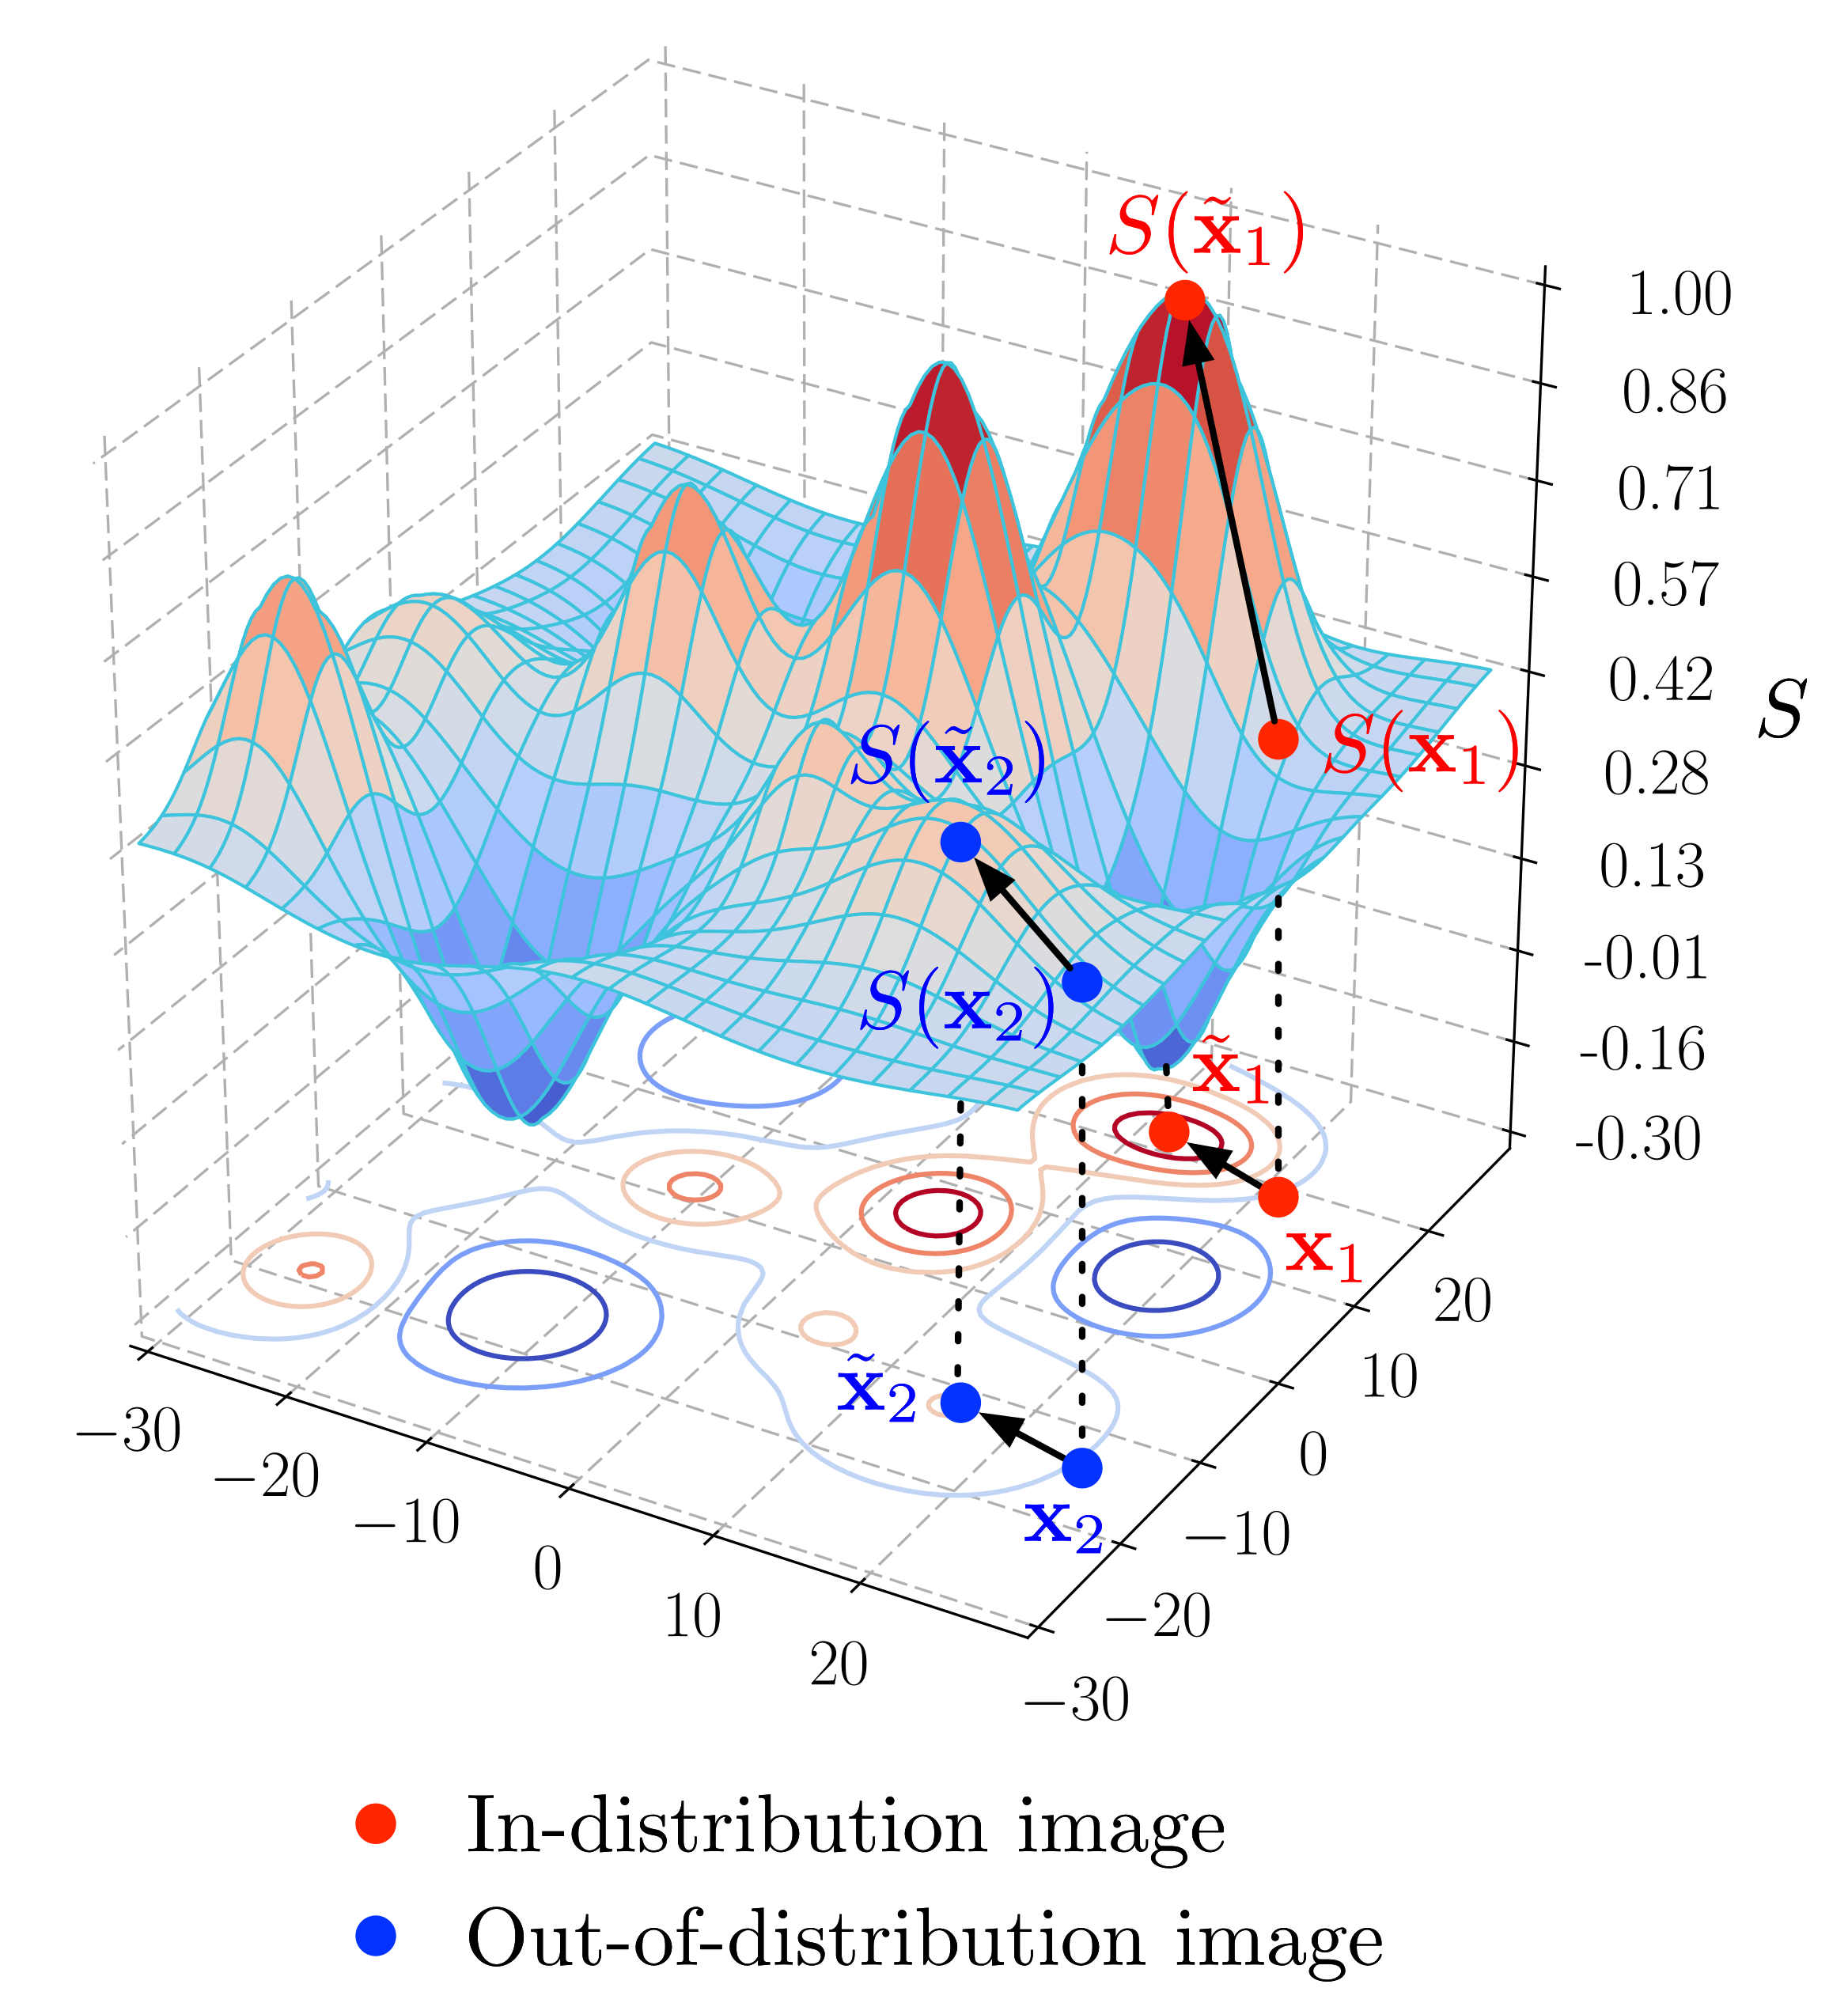
\includegraphics[width=3.25in]{figure/gradient.png}}
\caption{Figure taken from \cite{odin}, showing the difference in gradients between ID and OOD data points}
\label{softmaxmove}
\end{figure}

The interpretation of the temperature scaling is slightly more complex. By performing a Taylor expansion and omitting third and higher orders, we can rewrite the softmax score (i.e the value of the predicted class, the highest value) as ${S\propto {(U_{1}-U_{2}/2T)/T}}$, with $U_1$ and $U_2$ defined as follows \cite[4]{odin}:


\begin{equation}\label{eq::u1u2}
U_{1}(\bm{x})=\frac{1}{N-1}\sum_{i\neq\hat{y}}[f_{\hat{y}}(\bm{x})-f_{i}(\bm{x})]
\end{equation}

\begin{equation}\label{eq::u1u2}
U_{2}(\bm{x})=\frac{1}{N-1}\sum_{i\neq\hat{y}}[f_{\hat{y}}(\bm{x})-f_{i}(\bm{x})]^{2}
\end{equation}

$\hat{y}$ is the predicted class, and is thus also the index for the highest value in $f(\bm{x})$. Thus, $U_1$ represents "the extent to which the largest unnormalized output deviates from the remaining outputs", while $U_2$ measures how the remaining outputs deviate from each other \cite[6]{odin}.

\cite{odin} makes the two following observations with regards to these two values: Firstly, they find that the largest unnormalized output tends to deviate more for ID samples, making $U_1$ larger than for OOD samples, because the model is more confident in its prediction. Secondly, they find that $E[U_2|U_1]$ is larger for ID data samples than for OOD samples, which shows that ID samples have more separation in the remaining unnormalized inputs than OOD samples. 

Returning to the Taylor approximated softmax score ${S\propto {(U_{1}-U_{2}/2T)/T}}$, we see that $U_1$ contributes to making the softmax score higher, while $U_2$ reduces the softmax score. Given that both these values are higher for ID data, we will want to reduce the impact of $U_2$ and increase the impact of $U_1$. As $U_1$ is divided by $T$, while $U_2$ is divided by $2T^2$, increasing the temperature achieves this, as $U_2$ will decrease much faster than $U_1$. Thus, we can see how an increased temperature increases the softmax scores for ID data, and thus increases the gap between softmax scores for ID and OOD samples, making them easier to differentiate.

With these two modifications to the simple baseline proposed by \cite{oodbaseline}, \cite{odin} manages to increase the gap between the softmax scores of ID and OOD data and thus facilitates much more effective OOD detection.
\\

\subsubsection{Energy Based OOD Detection}

\cite{energy} proposes using an {\it energy score} as opposed to the softmax score. They show mathematically that "the softmax confidence score is a biased scoring function that is not aligned with the density of the inputs" \cite{energy}, and thus seek to use a different measurement which is better aligned with the probability density.

An energy function is a function $E(\bm{x}) : \mathbb{R}^D \rightarrow \mathbb{R}$ which maps any data point into a non-probabilistic scalar called energy. Energy values can be converted to probabilities using the Gibbs distribution defined below (equation \ref{energy}):

\begin{equation} \label{energy}
    p(y \mid \*x) = \frac{e^{-E(\*x,y)/T}}{\int_{y'} e^{-E(\*x, y')/T}}
    = \frac{e^{-E(\*x,y)/T}}{e^{-E(\*x)/T}},
\end{equation}

This equation is quite similar to the softmax function, and we can see that by defining $E(\bm{x}, y) = -f_y(x)$. We can write the Gibbs distribution as the normal softmax output of a neural network:

\begin{equation}\label{eq:softmax}
    p(y \mid \*x) = \frac{e^{f_y(\*x)/T}}{\sum_{i}^K e^{f_{i}(\*x)/T}},
\end{equation}

By using the {\it Helmholtz free energy} measurement, we can get an energy score for each data point given to the model, which can be used to detect OOD data points. Given that we define $E(\bm{x}, y) = -f_y(x)$, we can write the Helmholtz free energy $E(\bm{x})$ as:

\begin{equation}\label{eq:energy_softmax}
  E(\*x;f)=- T\cdot \text{log}\sum_i^K e^{f_i(\*x)/T}.
\end{equation}

The authors show that when training with negative log likelihood loss, the optimization will reduce the free energy of ID data points, and that the difference  between ID and OOD energy scores is higher than the difference in softmax scores \cite{energy}. Thus, thresholding the free energy function is an effective way to separate ID and OOD data points. Furthermore, they also present a method for fine tuning a pre trained model using a loss function that is based on the energy score. By doing this, the gap between ID and OOD energy scores can be increased even further.
\\

\subsubsection{ReAct}

ReAct \cite{react} is a very simple method, which also aims to increase the difference in confidence scores between ID and OOD data. It does this by rectifying high activations in the penultimate layer, which surprisingly achieves this very effectively. Figure \ref{react} gives an intuition for why this is the case:

\begin{figure}[h]
\centerline{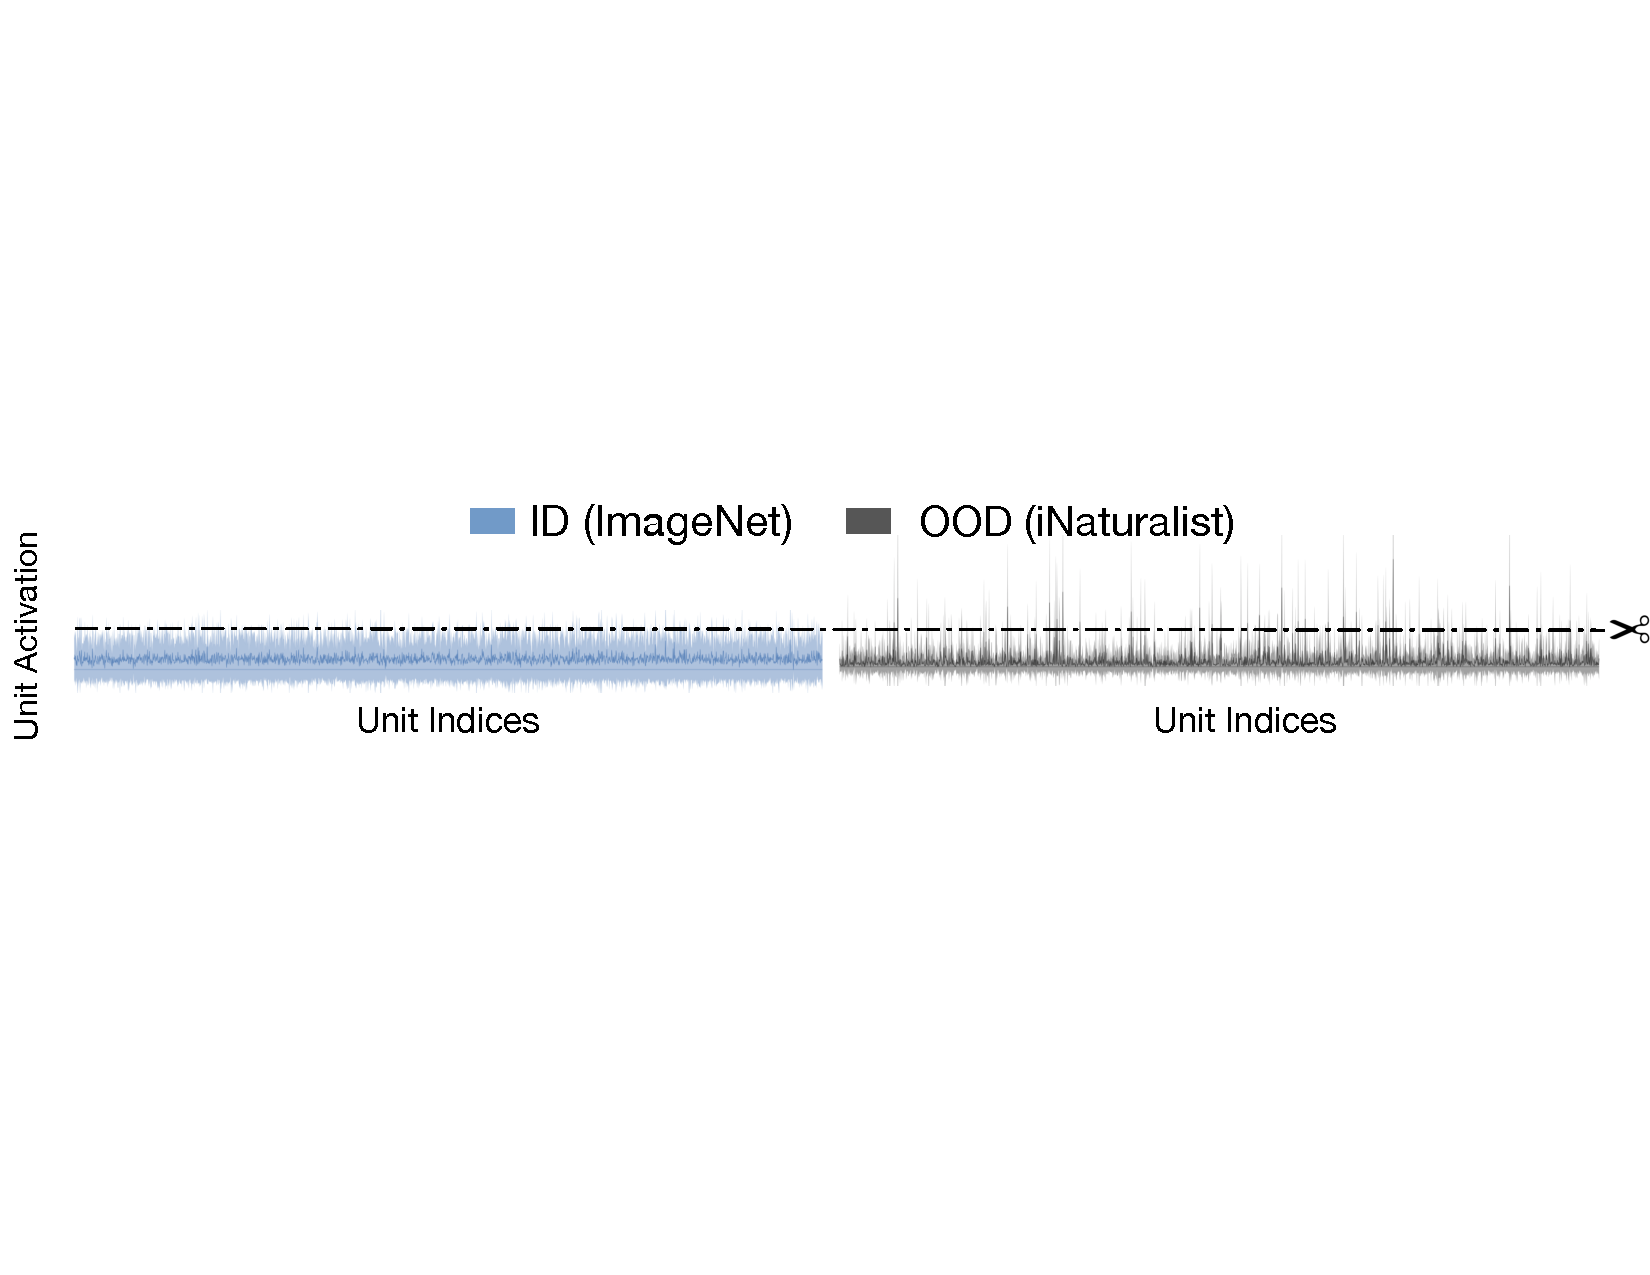
\includegraphics[width=3.25in]{figure/react.pdf}}
\caption{Figure taken from \cite{react}, showing the activations for the nodes in the penultimate layer for ID and OOD data}
\label{react}
\end{figure}

From this, we see that OOD samples have much more irregular activations, with a higher variance and many high value outliers. This gives an explanation for why OOD samples produce highly confident softmax scores: sharp positive outliers manifest in the model output, producing high logits in the output layer \cite{react}. By using a positive upper limit to rectify these outliers, we can remove their impact and reduce the confidence for OOD data.

This gives rise to a very simple OOD detector: Let us denote the feature vector of the penultimate layer as $h(\bm{x})$, where $\bm{x}$ is the input feature vector. The logits of the network would be calculated by the function

\begin{equation}\label{dog}
  f(\bm{x}) = W \, h(\bm{x}) + \bm{b},
\end{equation}

where $W$ is a matrix which projects $h(\bm{x})$ down to the output space. $h(\bm{x})$ is the vector which contains the high activations for OOD data, so by rectifying this vector with $\text{ReAct}(\bm{x}; c) = min(\bm{x}, c)$ for a $c > 0$, we can remove these outlier activations. We then get

\begin{equation}\label{dog}
  \bar{h}(\bm{x}) = \text{ReAct}(h(\bm{x}; c),
\end{equation}

which gives us the new output logits 

\begin{align}
f^{\text{ReAct}}(\*x;\theta) = \*W^\top \bar h(\*x) + \mathbf{b}.
\end{align}

These logits can be used by any other OOD method which uses the output values to separate ID and OOD samples \cite{react}:

\begin{align}
\label{eq:threshold}
	G_{\lambda}(\*x; f^\text{ReAct})=\begin{cases} 
      \text{in } & S(\*x;f^\text{ReAct})\ge \lambda \\
      \text{out} & S(\*x;f^\text{ReAct}) < \lambda 
   \end{cases},
\end{align}

This simple methods performs well on many benchmarks, with the added benefit that it can be combined with many other methods. For example, we can use ODIN or Energy with output scores calculated using ReAct instead of unrectified outputs, which leads to improvements over the methods used by themselves.
\\

\subsubsection{Virtual Outlier Synthesis (VOS)}

Generating outliers to expose to the model during training is another way to reduce the model's confidence on OOD data. However, creating realistic OOD data points can be difficult, especially if the input space is of a high dimension, such as in image classification. \cite{vos} presents a more tractable method, which synthesizes outliers not in the input space, but in the feature space, which can be of a much lower dimensionality.

In this lower dimension space, previously intractable methods are now less computationally expensive. To synthesize outliers, \cite{vos} simply estimate class conditional Gaussian distributions by computing empirical class means and covariances, and sample outliers from the class boundaries between these Gaussians.

Using these outliers, they present a "unknown-aware training objective", which can be used during training to maximize the separability between ID and OOD data during inference.
\\

\subsubsection{GradNorm}

As opposed to using the feature or output space, GradNorm \cite{gradnorm} attempts to use the gradient space of a network to calculate OOD-ness. They find that the gradients of the weights actually contain valuable information that allows for effective separation of ID and OOD samples, and perform ablation studies which show that this methods outperforms many other methods, including the previously mentioned ODIN and Energy methods.

The gradients are calculated with regards to the Kullback-Leibler divergence between the softmax values and a uniform distribution. An important distinction from other methods is that all the softmax values are used, as opposed to the {\it softmax score} which would be only the score of the predicted class. Thus, this method captures information about the uncertainty across all categories, as opposed to just the most likely class \cite[3]{gradnorm}. Once the gradients have been calculated, the threshold is simply done on the $L_p$-norm of these gradients, giving us the following thresholding function \cite{gradnorm}:

\begin{equation}
\label{eq:score}
    S(\*x) = \lVert\frac{\partial D_\text{KL}(\*u~\lVert~\text{softmax}(f(\*x))}{\partial \*w}  \rVert_p
\end{equation}

As shown in figure \ref{gradnorms}, we see that the gradient norms are consistently lower for OOD data (gray) than ID data (blue).

\begin{figure}[h]
\centerline{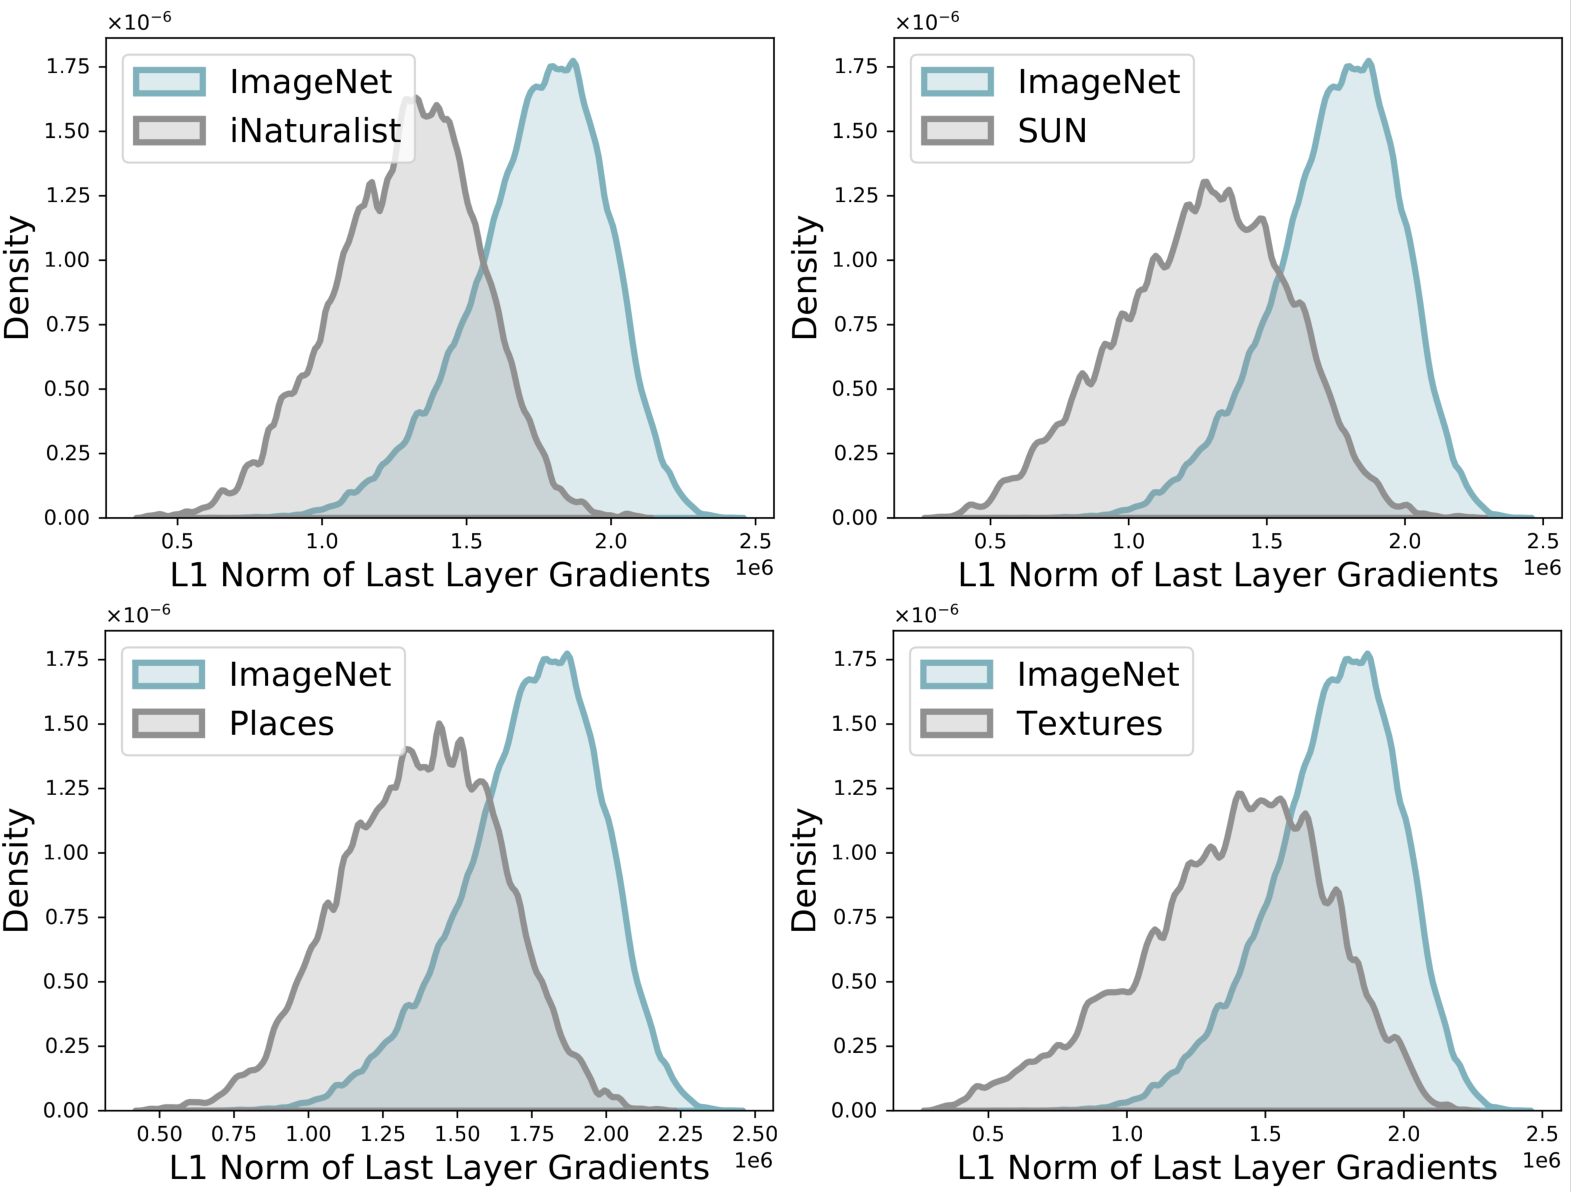
\includegraphics[width=3.25in]{figure/gradnorm.pdf}}
\caption{Figure taken from \cite{gradnorm}, showing the difference in gradient norms between ID and OOD data}
\label{gradnorms}
\end{figure}

\cite{gradnorm} find that it is sufficient to only calculate the gradients for the last layer of the network, and that the $L_1$-norm performs the best, as it weights all gradients equally, as opposed to higher norms which place more importance on larger values.

In their mathematical analysis, they show that GradNorm captures joint information from both the feature and output space. By decomposing the $L_1$-norm of gradients of weights of the last layer with regards to the Kullback-Leibler divergence, they reach the following equality:

\begin{equation}
S(\bm{x}) = \frac{1}{CT}  \left(\sum_{i=1}^m |x_i|\right) \left(\sum_{j=1}^C \left|1 - C \cdot \frac{e^{f_j / T}}{\sum_{j=1}^C e^{{f_{j}} / T}}\right|\right)
\label{eq:decomp}
\end{equation}

From this, we see that $S(\bm{x})$ is a product of a factor which is simply the $L_1$-norm of the feature vector $\bm{x}$, and another term which captures information about the softmax values in the output space.
\\

\subsubsection{Virtual Logit Matching (ViM)}

\cite{vim} attempts to improve OOD detection by calculating a score based on the feature, the logit and the softmax probability at once, as opposed to just one of them. By looking at all three elements in conjunction, they see an increase in performance over models which only rely on a single input source (such as the previously mentioned ODIN).

The reasoning behind not just looking at the logits or softmax probability is that there is a lot of information that is lost when going from features to logits \cite{vim}. Once we project the features down to logits, we have only class dependent information, and have lost the class agnostic information which is contained within the features. To show how this information is lost, the authors give an example based on null space analysis \cite{nusa}:

Let us assume that we have a simplified network with only a single layer. Then, we have $\hat{\bm{y}} = W \bm{x}$, where $\hat{\bm{y}}$ is the vector containing the logits, $\bm{x}$ is the feature vector of the input (with an additional 1 for the bias term) and $W$ is the matrix containing the weights and biases transforming the feature vector into logits. A null space $\text{Null}(W)$ of a matrix $W$ is the set of all vectors that map to the zero vector, such that $W \bm{a} = \bm{0} \iff \bm{a} \in \text{Null}(W)$. The null space of a matrix may be trivial (empty), but a matrix which projects vectors to a lower dimension have non-trivial null spaces. Given that the final layer of a neural network projects down to logits, which are the same dimension as the number of classes, this will almost always be the case. Because of the distributivity of matrix multiplication, we have the following:

\begin{equation}
W (\bm{x} + \bm{a}) = W \bm{x} + W \bm{a} = W \bm{x} + \bm{0} = W \bm{x}
\label{matrix}
\end{equation}

The vector $\bm{x}$ can be decomposed into $\bm{x}^W + \bm{x}^{\text{Null}(W)}$, where $\bm{x}^W$ is the projection of $\bm{x}$ onto the column space of $W$ and $\bm{x}^{\text{Null}(W)}$ is the projection of $\bm{x}$ onto the null space of $W$. It follows from this and equation \ref{matrix} that when going from features to logits using the projection $W \bm{x}$, we lose all information contained in $\bm{x}^{\text{Null}(W)}$. \cite{nusa} shows how this can be exploited by adversarial methods, by creating images with added noise derived from the null space of a matrix within the network, which are classified as if the noise was not present, despite having no resemblance to the original image. See figure \ref{dog}.

\begin{figure}[hbt]
    \centering
    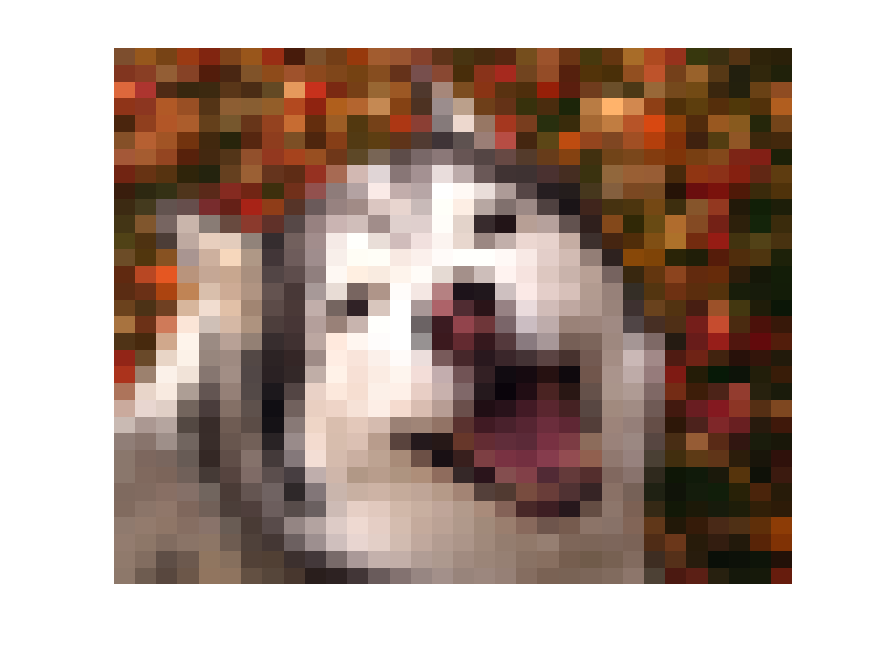
\includegraphics[width=0.32\linewidth,trim={1.25cm 1.25cm 1.25cm 1.25cm},clip]{figure/OrigImage.pdf}
    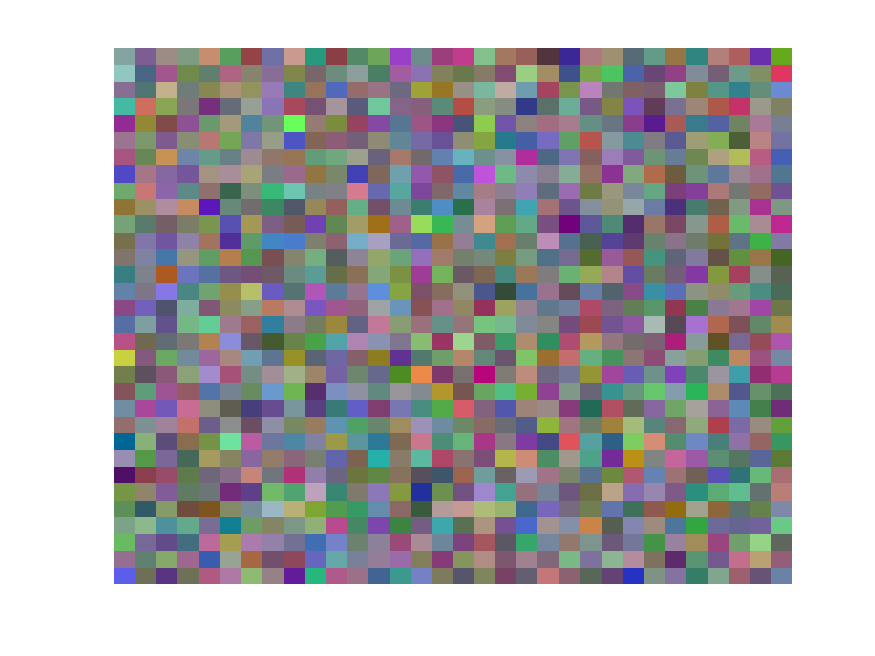
\includegraphics[width=0.32\linewidth,trim={1.25cm 1.25cm 1.25cm 1.25cm},clip]{figure/PureNoise.pdf}
    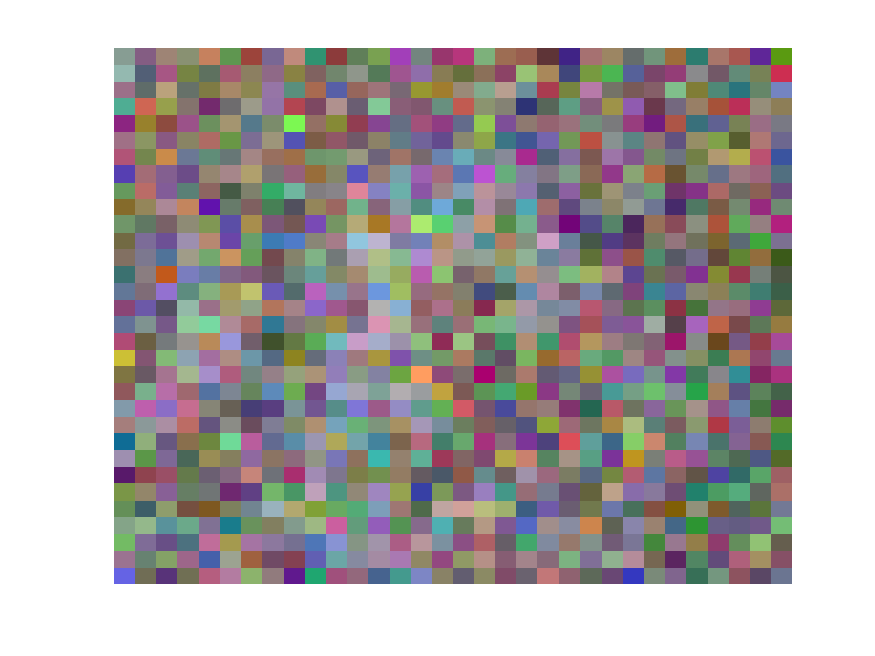
\includegraphics[width=0.32\linewidth,trim={1.25cm 1.25cm 1.25cm 1.25cm},clip]{figure/NoiseAdded.pdf}
    \caption{Image taken from \cite{nusa}. Left: Original image. Center: Additive null space noise. Right: Final image, indistinguishable from original image according to the network the noise in the center column is sampled from.}
    \label{dog}
\end{figure}

From this, we can see that potentially large amounts of information can be lost when going from features to logits. Using this information, it is also possible to perform OOD detection, as shown by \cite{nusa}. Another method which uses the features performs Principal Component Analysis (PCA) and looks at the residual information lost when using the first $N$ principal components \cite{subspace}. However, the information in the features is still class agnostic, and \cite{vim} aims to go beyond using just one input source and combine several elements of the network.

To do this, they propose using a {\it Virtual Logit}. The Virtual Logit is calculated as follows: First, they center the feature space, so that "it is bias free in the computation of logits" \cite{vim}. They then perform PCA as in \cite{subspace}, and calculate the residual of $\bm{x}$ with regards to the principal components, which is the projection $\bm{x}$ onto the null space of the principal subspace $P$. The residual represents the information lost when using the projection $P$.

\begin{equation}
\text{Residual}(x) = || \bm{x}^{\text{Null}(P)}||
\label{virtuallogit}
\end{equation}

This value is scaled based on the average values of the maximum logit across the dataset, and is appended to the rest of the logits as a Virtual Logit:

\begin{equation}
l_0 := \alpha || \bm{x}^{\text{Null}(P)}||
\label{virtuallogit}
\end{equation}

This now takes part in the computation of the softmax values, and thus is affected by the size of the rest of the logits. They call the softmax value of the Virtual Logit the {\it ViM score}. In this way, the ViM score represents the size of the residual in comparison with the predictions of the model. If the model is very confident, then the norm of the residual will be small in comparison, and the ViM score will be low. If the residual is very large, the ViM score will be higher, and more indicative of an OOD sample. In this way, \cite{vim} have combined information from the feature, the logit and the softmax probability level to perform OOD detection.

\chapter{New method} \label{chapter:newmethod}

\chapter{Experiments and Results} \label{chapter:experiments}

\chapter{Discussion} \label{chapter:discussion}

\chapter{Conclusion} \label{chapter:conclusion}

\section{Future work}



\backmatter{}
\printbibliography{}
\end{document}
